\begin{newpage}
  \section{Problemlösungsprozess}
  \label{sec:problemlösungsprozess}
    Dieses Kaptiel soll den durchlaufenen Prozess sowie die einzelnen Schritte beschreiben, die zur Realisierung des Projekts unternommen wurden. 

    Das Projekt wurde nach dem Design Prozess \texttt{"`The Double Diamond"'}\footnote{\url{http://www.designcouncil.org.uk/news-opinion/design-process-what-double-diamond}} bearbeitet. Der Double Diamond wurde vom British Design Council 2005 entwickelt und soll im folgenden danach beschrieben werden.\parencite{designcouncil}

    \begin{figure}[htbp]
      \begin{center}
        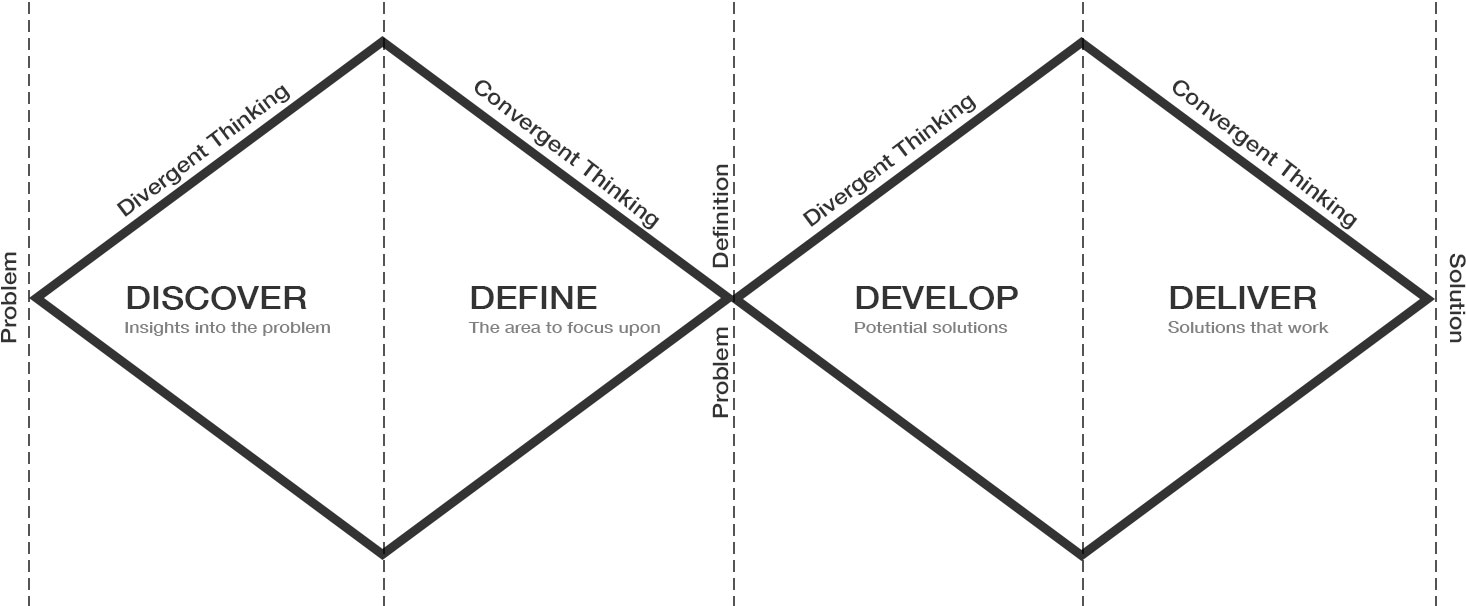
\includegraphics[width=0.9\textwidth]{double_diamond}
        \caption{"`The Double Diamond"' eigene Abbildung nach \parencite{designcouncil}}
        \label{fig:double_diamond}
      \end{center}
    \end{figure}

    Der Double Diamond beschreibt ein iterative Prozess. Wie in allen kreativen Prozessen werden dabei eine Reihe von möglichen Ideen geschaffen ("divergentes Denken"), bevor sie verfeinert und auf die beste Idee reduziert werden ("konvergentes Denken"). Der Double Diamond zeigt jedoch an, dass dies zweimal geschieht - einmal zur Bestätigung der Problemdefinition und einmal zur Erstellung der Lösung. Einer der größten Fehler ist es, den linken Diamanten wegzulassen und am Ende das falsche Problem zu lösen.

    \begin{itemize}[label={}]
      \item \textbf{Discover:} Der erste Teil des Double Diamond steht am Anfang des Projektes. Hier wird versucht, die Welt neu zu sehen, Neues wahrzunehmen und Einsichten in das zu lösende Problem zu sammeln.

      \item \textbf{Define:} Der zweite Teil stell die Definitionsphase dar. Dabei wird versucht alle in der Entdeckungsphase identifizierten Möglichkeiten zu verstehen. Ziel ist es dabei, ein klares Briefing zu entwickeln, das die grundsätzlichen Herausforderungen umrahmt.

      \item \textbf{Develop:} Der dritte Teil markiert eine Entwicklungsphase, in der Lösungen oder Konzepte erstellt, prototypisiert, getestet und iteriert werden. Dieser Prozess des Ausprobierens hilft, Ideen zu verbessern und zu verfeinern.

      \item \textbf{Deliver:} Der letzte Teil des Double Diamond ist die Lieferphase, in der das daraus resultierende Projekt (z. B. ein Produkt, eine Dienstleistung oder eine Umwelt) abgeschlossen, produziert und in Betrieb genommen wird.
    \end{itemize}
    

    \subsection{Discover}
    \label{sub:discover}
      Dafür erfolgte eine weitreichende Recherche zu relevanten Themenbereichen wie Live Visualisierung, Visualisierung von öffentlichem Nahverkehr sowie Tools zum Erstellen von Karten (Abbildung \ref{fig:viz_overview}). 

      \begin{figure}[ht]
        \begin{center}
          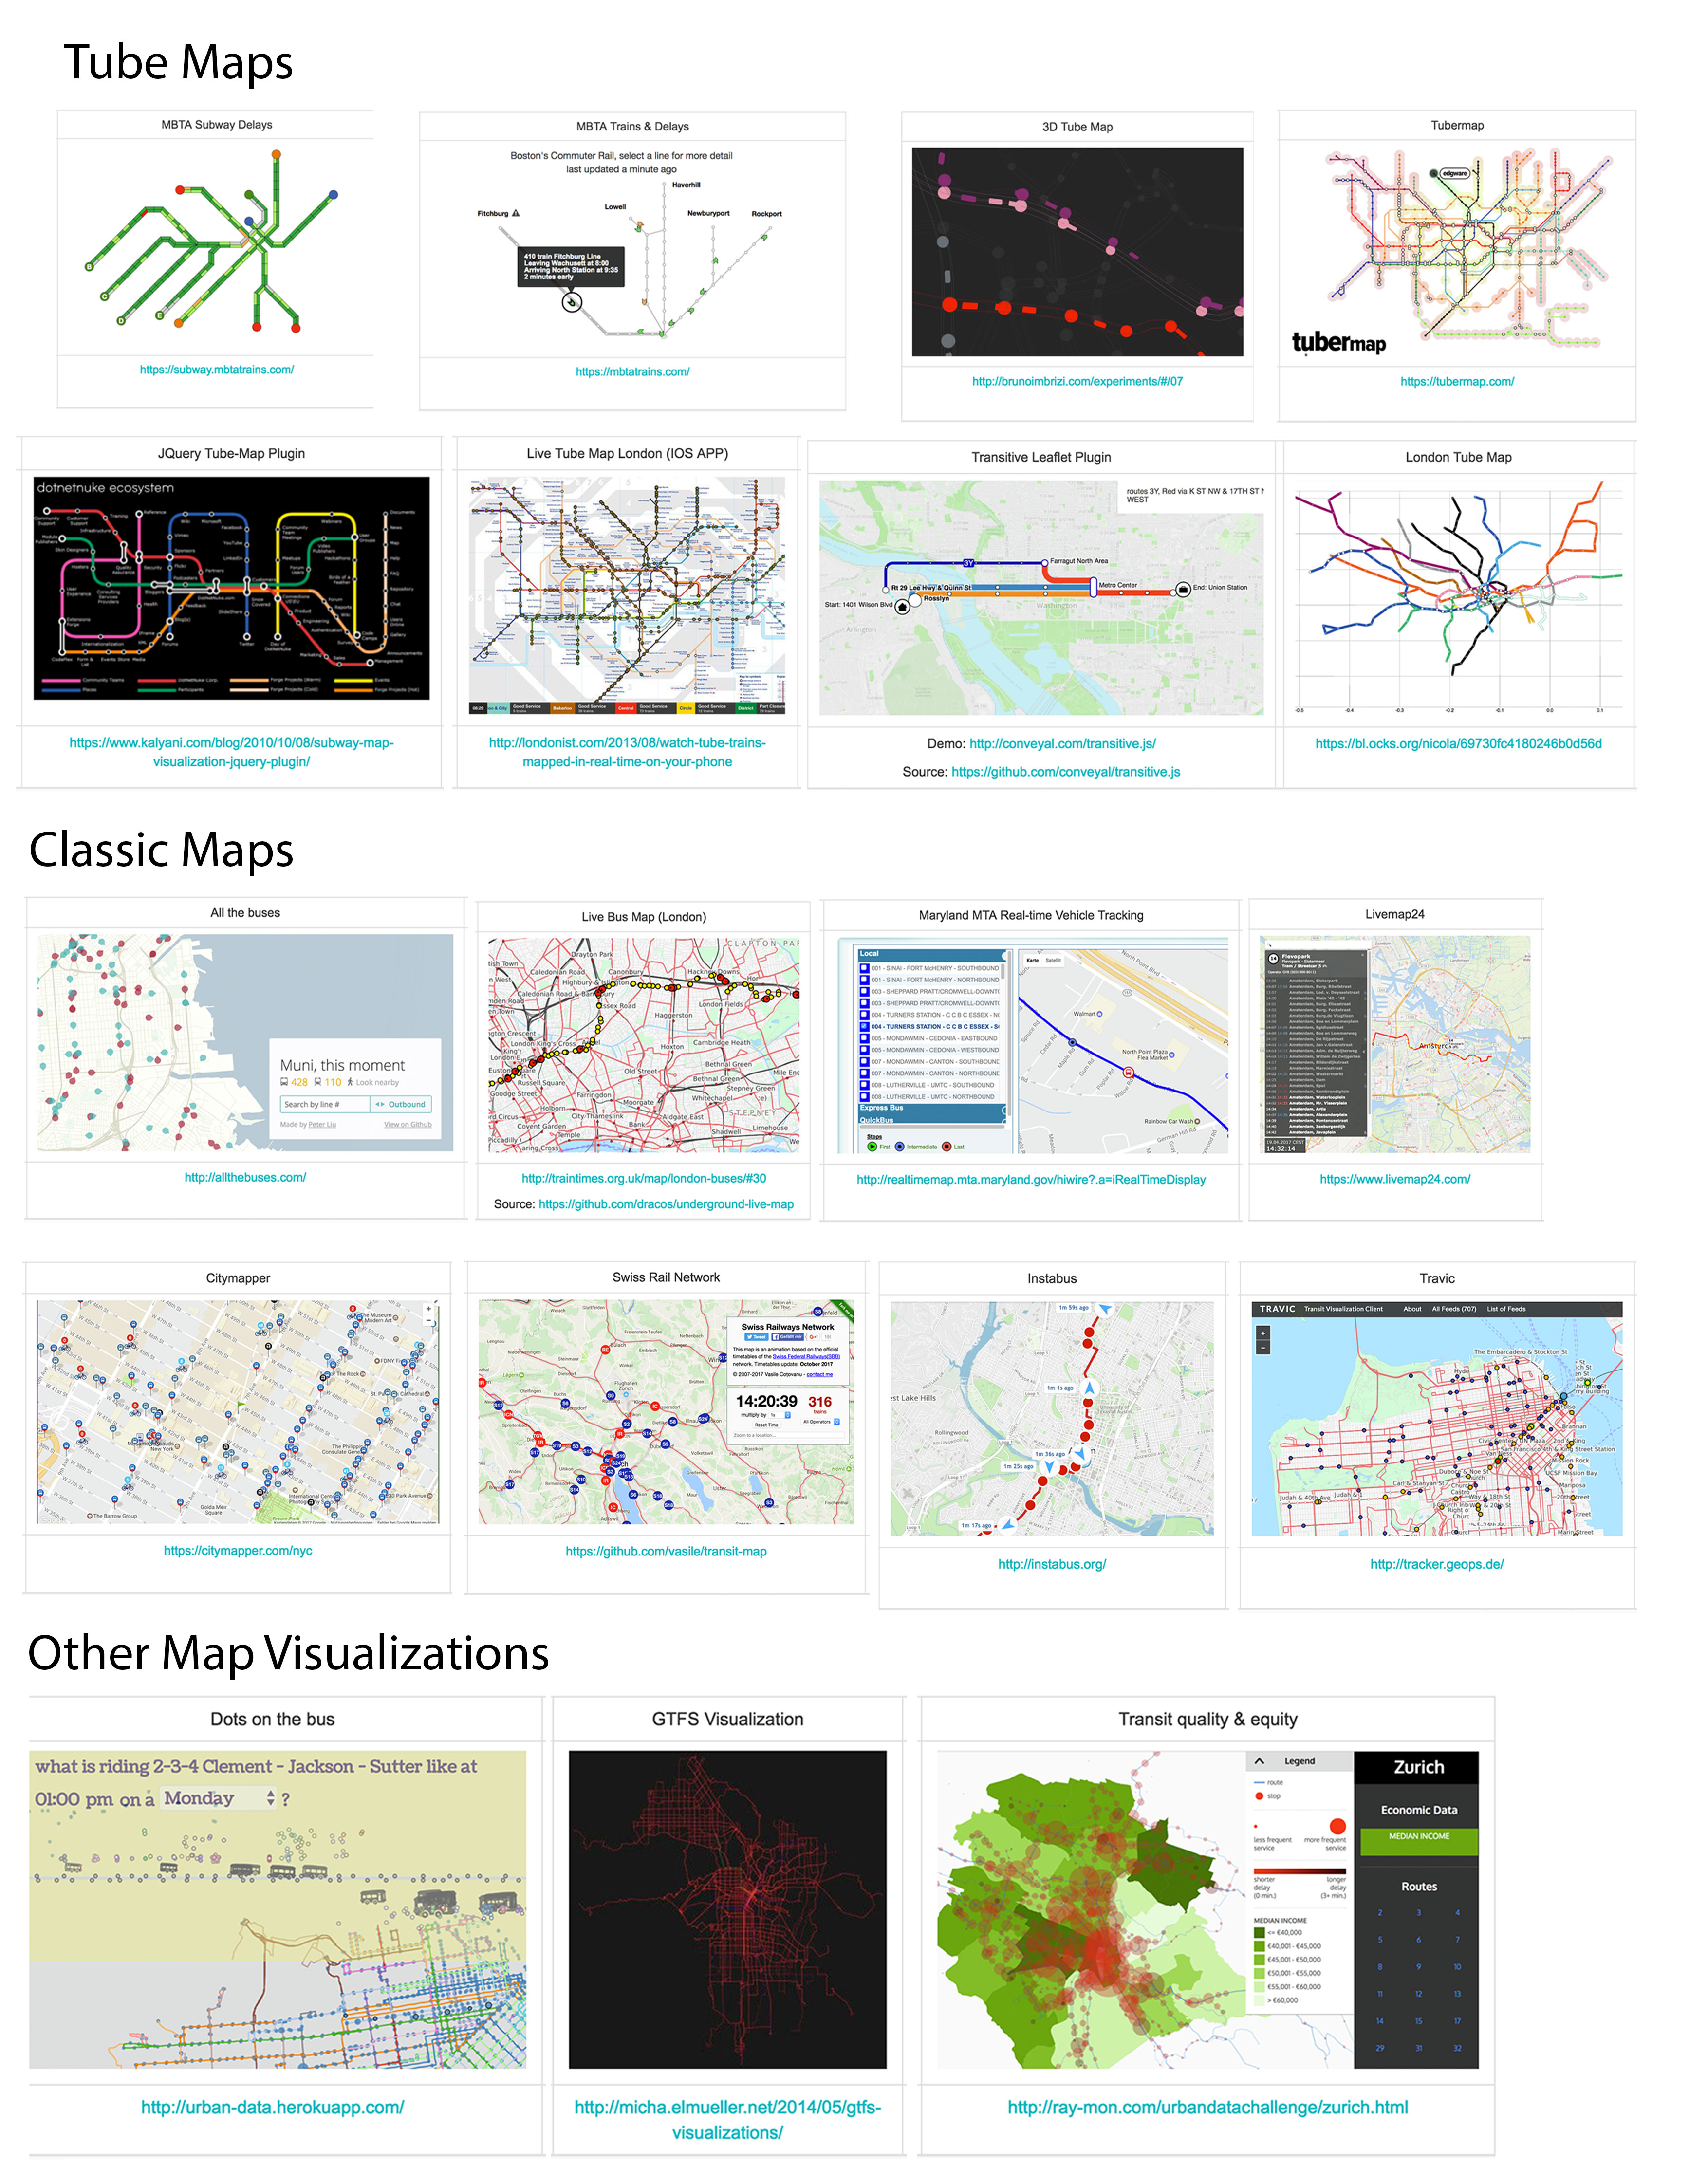
\includegraphics[width=0.80\textwidth]{viz_overview}
          \caption{Überblick über bestehende Tools und Visualisierungen}
          \label{fig:viz_overview}
        \end{center}
      \end{figure}

      Das gesammelte Material wurde in einer 2x2 Matrix (Abbildung \ref{fig:2x2_matrix}) in die Unterkategorien "`Live Map, Künstlerische Visualisierung, Plugin / Software / Tool, Tube-Map"' eingeordnet um einen sortierten Gesamtüberblick zu bekommen. 

      \begin{figure}[htbp]
        \begin{center}
          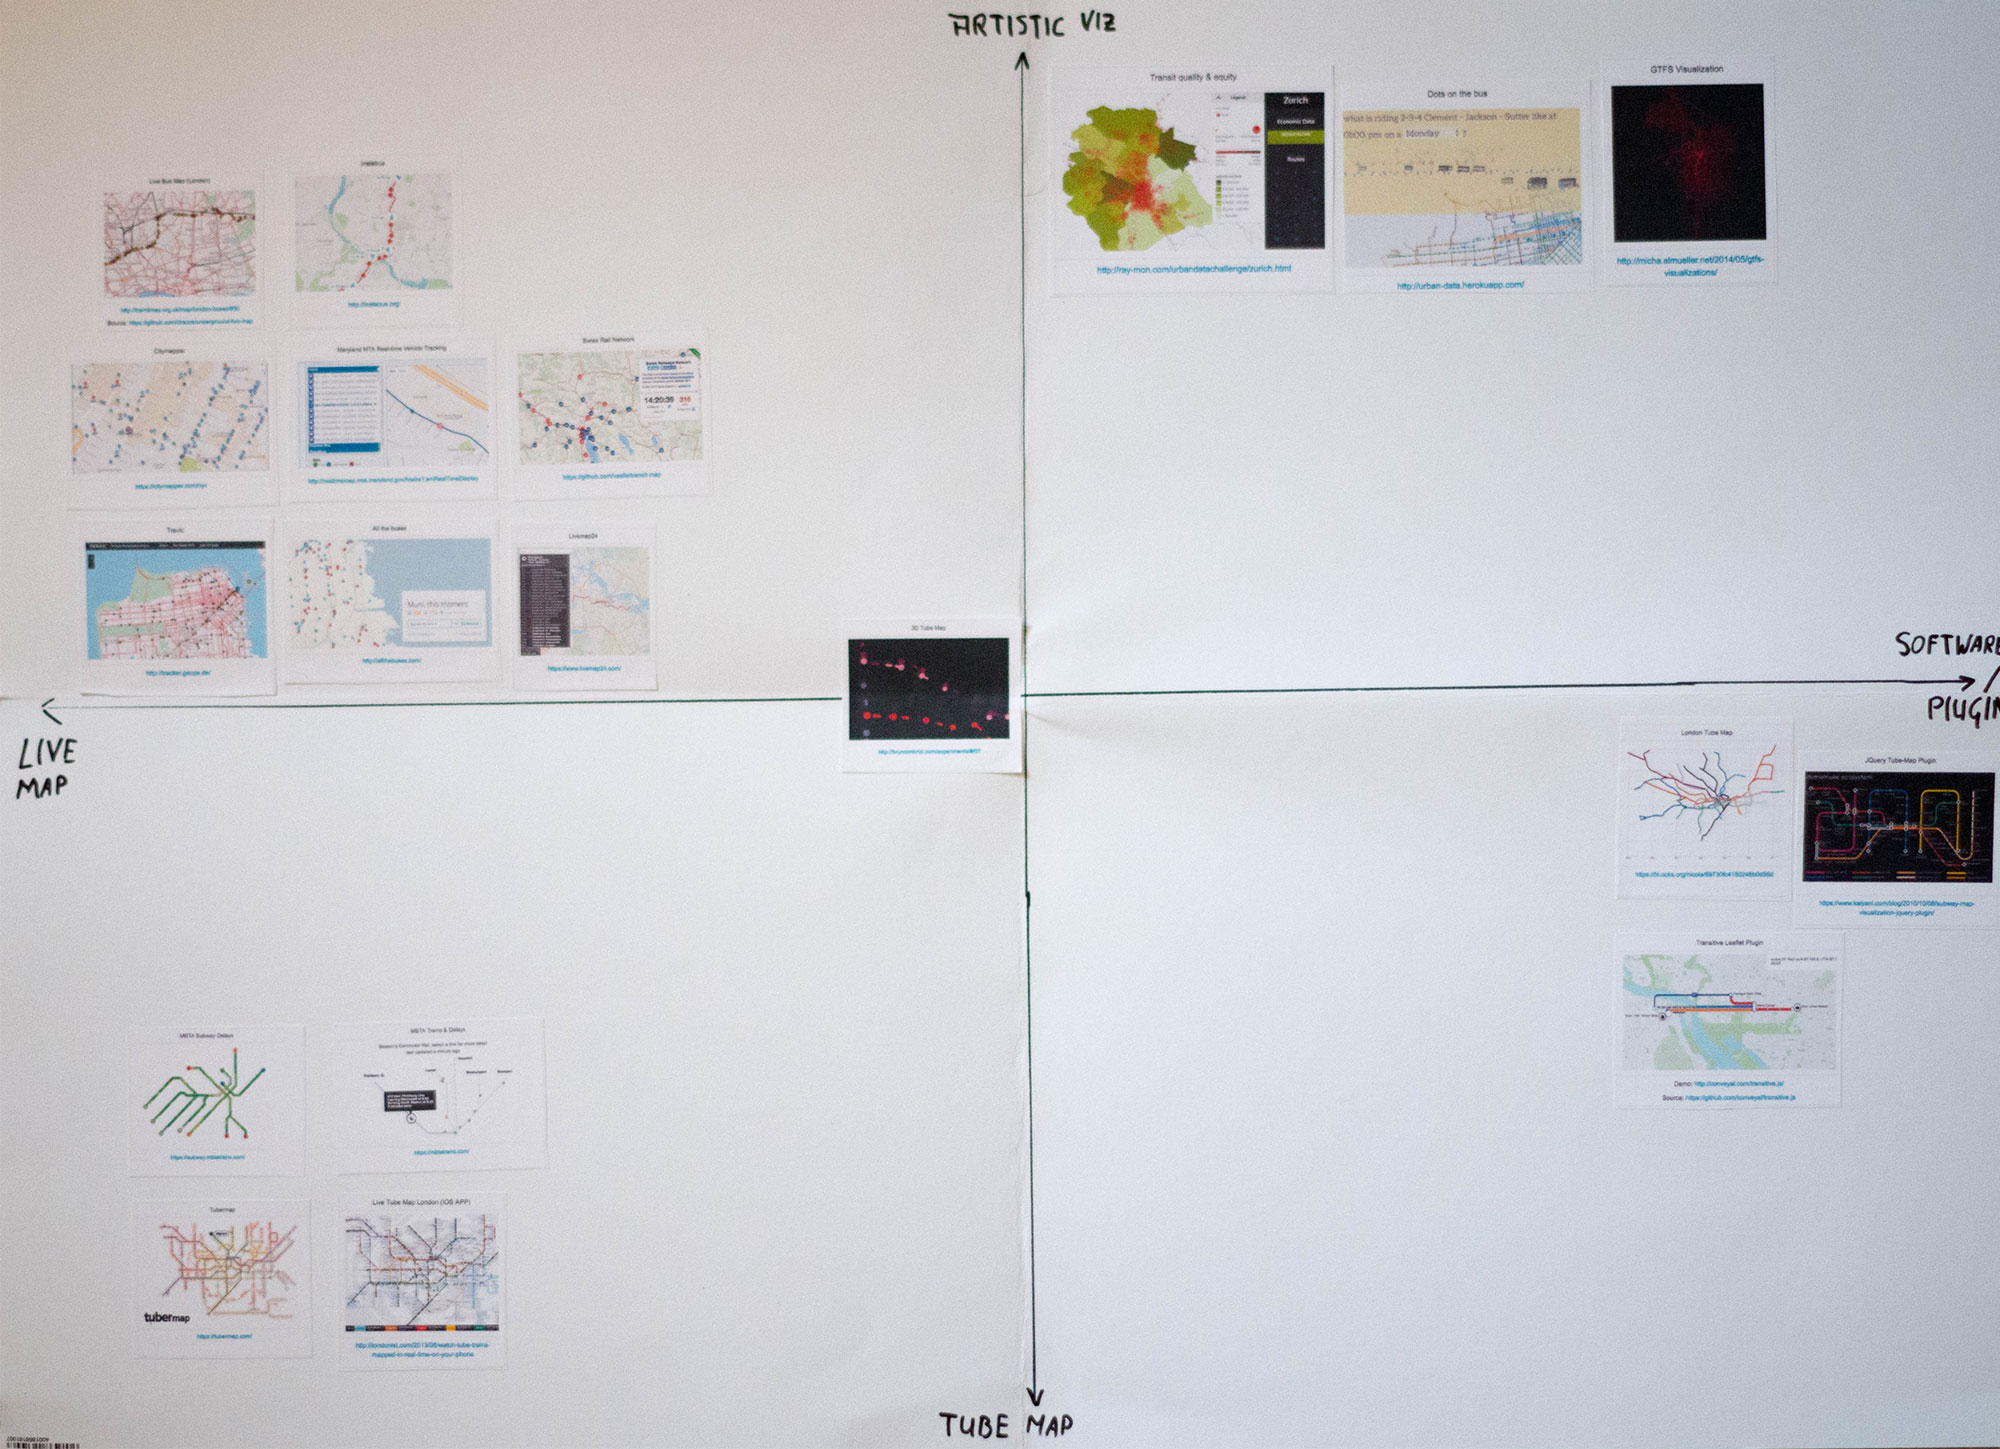
\includegraphics[width=0.5\textwidth]{2x2_matrix}
          \caption{2x2 Matrik Methode auf DIN A2}
          \label{fig:2x2_matrix}
        \end{center}
      \end{figure}

      Durch diese Ansicht wurde die Erkenntnis gewonnen, dass es schon viele Live Visualisierungen auf interaktiven Karten gibt, aber nur sehr wenig so genannten Tube-Maps. Der Ansatz die Visualisierung in Richtung einer Tube-Map zu entwickeln, oder gar ein kombinatorischer Ansatz zwischen Tube-Map und klassischer Karte, wurde diskutiert und als mögliches Ziel definiert. Aufgrund des Umfangs und der kurzen Zeitspanne einer Master-Thesis, konnte diese Richtung allerdings nicht näher verfolgt werden. Diese erste Phase nahm ungefähr 4 Wochen Zeit in anspruch.
      
    % subsection discover (end)

    \subsection{Define}
    \label{sub:define}
      
    % subsection define (end)

    \subsection{Develop}
    \label{sub:develop}
      
    % subsection develop (end)

    \subsection{Deliver}
    \label{sub:deliver}
      
    % subsection deliver (end)
  % \begin{itemize}
  %   \item Überblick verschaffen
  %   \item Recherche Phase -> related visualizations
  %   \item What is not done?
  %   \item Limiting own scope
  % \end{itemize}

  % \begin{itemize}
  %   \item Introduce step by step solutions
  %   \item Screenshots
  %   \item Mockups
  %   \item Solving problems by iterative process
  % \end{itemize}
    
  % section problemlösungsprozess (end)
\end{newpage}